\documentclass[a4paper,10pt]{article}
\usepackage[brazilian]{babel}
\usepackage[left=2.5cm,right=2.5cm,top=3cm,bottom=2.5cm]{geometry}
\usepackage{mathtools}
\usepackage{amsthm}
\usepackage{amsmath}
%\usepackage{nccmath}
\usepackage{amssymb}
\usepackage{amsfonts}
\usepackage{physics}
%\usepackage{dsfont}
%\usepackage{mathrsfs}

\usepackage{titling}
\usepackage{indentfirst}

\usepackage{bm}
\usepackage[dvipsnames]{xcolor}
\usepackage{cancel}

\usepackage{xurl}
\usepackage[colorlinks=true]{hyperref}

\usepackage{float}
\usepackage{graphicx}
%\usepackage{tikz}
\usepackage{caption}
\usepackage{subcaption}

%%%%%%%%%%%%%%%%%%%%%%%%%%%%%%%%%%%%%%%%%%%%%%%%%%%

\newcommand{\eps}{\epsilon}
\newcommand{\vphi}{\varphi}
\newcommand{\cte}{\text{cte}}

\newcommand{\N}{\mathbb{N}}
\newcommand{\Z}{\mathbb{Z}}
\newcommand{\Q}{\mathbb{Q}}
\newcommand{\R}{\vb{R}}
\newcommand{\C}{\mathbb{C}}
\renewcommand{\S}{\hat{S}}
%\renewcommand{\H}{\s{H}}

\renewcommand{\a}{\vb{a}}
\newcommand{\nn}{\hat{n}}
\renewcommand{\d}{\dagger}
\newcommand{\up}{\uparrow}
\newcommand{\down}{\downarrow}

\newcommand{\0}{\vb{0}}
%\newcommand{\1}{\mathds{1}}
\newcommand{\E}{\vb{E}}
\newcommand{\B}{\vb{B}}
\renewcommand{\v}{\vb{v}}
\renewcommand{\r}{\vb{r}}
\renewcommand{\k}{\vb{k}}
\newcommand{\p}{\vb{p}}
\newcommand{\q}{\vb{q}}
\newcommand{\F}{\vb{F}}

\newcommand{\s}{\sigma}
%\newcommand{\prodint}[2]{\left\langle #1 , #2 \right\rangle}
\newcommand{\cc}[1]{\overline{#1}}
\newcommand{\Eval}[3]{\eval{\left( #1 \right)}_{#2}^{#3}}

\newcommand{\unit}[1]{\; \mathrm{#1}}

\newcommand{\n}{\medskip}
\newcommand{\e}{\quad \mathrm{e} \quad}
\newcommand{\ou}{\quad \mathrm{ou} \quad}
\newcommand{\virg}{\, , \;}
\newcommand{\ptodo}{\forall \,}
\renewcommand{\implies}{\; \Rightarrow \;}
%\newcommand{\eqname}[1]{\tag*{#1}} % Tag equation with name

\setlength{\droptitle}{-7em}

\theoremstyle{plain}
\newtheorem{theorem}{Teorema}[section]
%\newtheorem{defi}[theorem]{Definição}
\newtheorem{lemma}[theorem]{Lema}
%\newtheorem{corol}[theorem]{Corolário}
%\newtheorem{prop}[theorem]{Proposição}
%\newtheorem{example}{Exemplo}
%
%\newtheorem{inneraxiom}{Axioma}
%\newenvironment{axioma}[1]
%  {\renewcommand\theinneraxiom{#1}\inneraxiom}
%  {\endinneraxiom}
%
%\newtheorem{innerpostulado}{Postulado}
%\newenvironment{postulado}[1]
%  {\renewcommand\theinnerpostulado{#1}\innerpostulado}
%  {\endinnerpostulado}
%
%\newtheorem{innerexercise}{Exercício}
%\newenvironment{exercise}[1]
%  {\renewcommand\theinnerexercise{#1}\innerexercise}
%  {\endinnerexercise}
%
%\newtheorem{innerthm}{Teorema}
%\newenvironment{teorema}[1]
%  {\renewcommand\theinnerthm{#1}\innerthm}
%  {\endinnerthm}
%
\newtheorem{innerlema}{Lema}
\newenvironment{lema}[1]
  {\renewcommand\theinnerlema{#1}\innerlema}
  {\endinnerlema}
%
%\theoremstyle{remark}
%\newtheorem*{hint}{Dica}
%\newtheorem*{notation}{Notação}
%\newtheorem*{obs}{Observação}


\setlength\parindent{0pt}  % noindent in entire file

\usepackage{minted}
\usemintedstyle{vs}
\definecolor{bg}{rgb}{0.85,0.85,0.85}
\setmintedinline{bgcolor=bg}
\newcommand{\python}[1]{\mintinline{python}{#1}}
\usepackage{tcolorbox}
\tcbuselibrary{minted,skins}
\newtcblisting{Python}{
  listing engine=minted,
  colback=bg,
  colframe=black!70,
  listing only,
  minted style=vs,
  minted language=python,
  minted options={texcl=true},
  left=1mm,
}

\newcommand{\lr}{\leftrightarrow}

\title{\Huge{\textbf{Teoria de grupos - Exercício 2}}}
\author{Mateus Marques}


\begin{document}

\maketitle

Minha abordagem para este exercício será computacional. Irei gerar as tabelas de multiplicação através de programação orientada a objetos no \python{python}. Para isso definirei \python{class Element}, associada aos elementos do grupo em questão, que serão definidos de acordo com permutações da \python{class Perm}.

O código source completo do meu programa está disponível no final deste documento.


\section*{1. Etano eclipsado C$_2$H$_6$}

\begin{figure}[H]
\centering
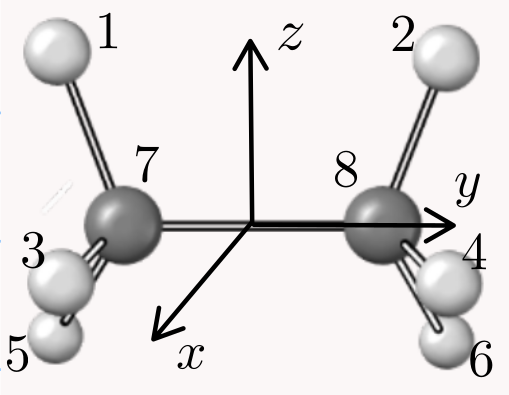
\includegraphics[width=0.3\linewidth]{fig/etano_eclipsado.png}
\caption{Etano eclipsado C$_2$H$_6$ com seus átomos enumerados.}
\label{fig:etano_eclipsado}
\end{figure}

Para o etano eclipsado, nós labelamos seus átomos de hidrogênio com os números $1,2,3,4,5,6$ e seus átomos de carbono com os números $7,8$, de acordo com a Figura \ref{fig:etano_eclipsado}. A título de exemplo, então podemos definir a permutação identidade $E$ e a reflexão $\sigma_h$ (no plano $xz$).
\begin{equation} \label{eq:E-Sigma_h}
E =
\begin{pmatrix}
1 & 2 & 3 & 4 & 5 & 6 & 7 & 8 \\
1 & 2 & 3 & 4 & 5 & 6 & 7 & 8 \\
\end{pmatrix}
\e
\sigma_h =
\begin{pmatrix}
1 & 2 & 3 & 4 & 5 & 6 & 7 & 8 \\
2 & 1 & 4 & 3 & 6 & 5 & 8 & 7 \\
\end{pmatrix}.
\end{equation}
Isso pois a reflexão $\sigma_h$ troca $1 \lr 2$, $3 \lr 4$, $5 \lr 6$ e $7 \lr 8$. No caso de nossa implementação no \python{python}, o que faremos é associar esses dois elementos $E$ e $\sigma_h$ às listas (definida dentro da \python{class Perm})
\begin{Python}
Perm([1,2,3,4,5,6,7,8])     # para o elemento identidade $E$
Perm([2,1,4,3,6,5,8,7])     # para a reflexão $\sigma_h$
\end{Python}
que são essencialmente a segunda linha das matrizes da equação \ref{eq:E-Sigma_h}.

A definição da \python{class Perm} é
\begin{Python}
class Perm:
    def __init__(self, L):  # inicialização a partir de uma lista
        self.n = len(L)     # tamanho da lista
        self.list = [i-1 for i in L]  # subtrair 1 para indexar a partir do zero
    def __eq__(self, other):
        return self.list == other.list  # são iguais se as listas são iguais
    def __mul__(self, other):  # multiplicação de duas permutações
        return Perm([self.list[i]+1 for i in other.list])  # composição
    def find(self, j):  # método auxiliar para achar a posição de um número na lista
        for i in range(self.n):
            if self.list[i] == j:
                return i
    def inv(self):  # calcula a inversa de uma permutação
        return Perm([self.find(j)+1 for j in range(self.n)])
\end{Python}

O método \python{__mul__(self, other)} define como é a multiplicação de dois elementos. Para exemplificar, considere as permutações do triângulo $A$ e $B$, definidas por
$$
A = C_3 =
\begin{pmatrix}
1 & 2 & 3 \\
2 & 3 & 1
\end{pmatrix}
\e
B = \sigma_{\text{v}1} =
\begin{pmatrix}
1 & 2 & 3 \\
1 & 3 & 2
\end{pmatrix},
$$
que no \python{python} seriam definidas por
\begin{Python}
A = Perm([2,3,1])   # == Perm( [A[1], A[2], A[3]] )
B = Perm([1,3,2])   # == Perm( [B[1], B[2], B[3]] )
\end{Python}

Essas permutações têm como regras
$$
\begin{cases}
\; A: 1 \to 2, \; 2 \to 3, \; 3 \to 1; \\
\; B: 1 \to 1, \; 2 \to 3, \; 3 \to 2.
\end{cases}
$$

Portanto, a multiplicação é $BA: 1 \to 3, \; 2 \to 2, \; 3 \to 1$, sendo representada por
$$
BA = \sigma_{\text{v}2} =
\begin{pmatrix}
1 & 2 & 3 \\
3 & 2 & 1
\end{pmatrix},
$$
que no \python{python} seria
\begin{Python}
B*A = Perm([3,2,1])   # = Perm( [B[A[1]], B[A[2]], B[A[3]]] )
\end{Python}

Por isso o método \python{__mul__(self, other)} é definido como
\begin{Python}
def __mul__(self, other):
    return Perm([self.list[i]+1 for i in other.list])
\end{Python}

No fundo estamos fazendo a composição \python{[ B[A[i]] for i in [1,2,...] ]}. Um detalhe é que realizamos a soma \python{+1} devido ao \python{python} indexar os números a partir do zero.

A explicação acima do método \python{__mul__} é a essência de nossa implementação. Para calcularmos as propriedades do grupo $D_{3h}$ basta que definamos seus elementos com a \python{class Element}, que nada mais é que uma \textit{data structure} com a permutação \python{Perm} e o nome do elemento.
\begin{Python}
class Element:  # permutacao e o nome
    def __init__(self, perm, eqname):
        self.perm = perm
        self.name = eqname[1:-1]  # remove '\$\$' from latex equation
        self.eqname = eqname
\end{Python}

No caso, o atributo \python{Element.eqname} significa o código em \LaTeX \, do elemento em questão. Por exemplo, para o $\sigma_h$ seria \python{r'$\sigma_h$'}. Eu faço isso pois planejo fazer meu programa printar a tabela já em formato de \LaTeX.

Para gerar o grupo $D_{3h}$, lembre que ele se escreve como o produto direto
\begin{equation} \label{eq:D3h-direct}
D_{3h} = D_3 \otimes C_{1h} =
\{E, C_3, C_3^2, C_2^{(1)}, C_2^{(2)}, C_2^{(3)}\} \otimes \{E, \sigma_h\} =
\end{equation}
$$
=
\{E, C_3, \underbrace{C_3^2}_{C_3^{-1}}, C_2^{(1)}, C_2^{(2)}, C_2^{(3)},
\underbrace{\sigma_v^{(1)}}_{C_2^{(1)} \sigma_h},
\underbrace{\sigma_v^{(2)}}_{C_2^{(2)} \sigma_h},
\underbrace{\sigma_v^{(3)}}_{C_2^{(3)} \sigma_h},
\sigma_h,
\underbrace{S_3}_{C_3 \sigma_h},
\underbrace{S_3^2}_{C_3^2 \sigma_h}\}.
$$

Basta então definir os elementos $E, C_3, C_2^{(1)}, C_2^{(2)}, C_2^{(3)}, \sigma_h$. Os demais serão obtidos por operações do grupo a partir destes mencionados.

As permutações de $E$ e $\sigma_h$ já foram definidas anteriormente na equação \ref{eq:E-Sigma_h}. A rotação $C_3$ gira os átomos de hidrogênio no sentido anti-horário pelo eixo $y$ da Figura \ref{fig:etano_eclipsado}, na ordem $1 \to 3 \to 5 \to 1$ e $2 \to 4 \to 6 \to 2$. As três rotações $C_2^{(j)}$ trocam os átomos de acordo com a Figura \ref{fig:C2_eclipsado}.
\begin{figure}[H]
\centering
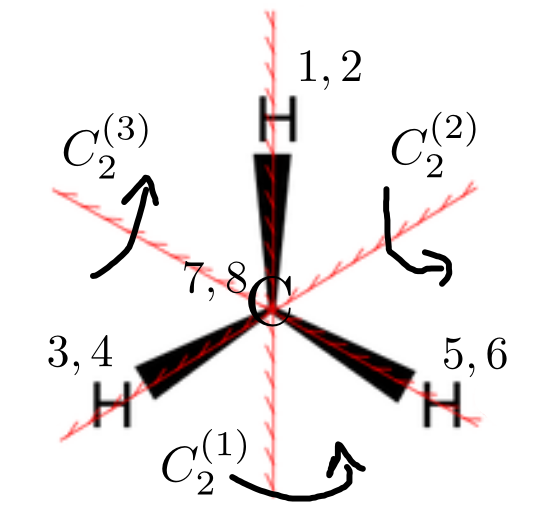
\includegraphics[width=0.3\linewidth]{fig/C2_eclipsado.png}
\caption{Eixos de rotação $C_2$ numa visão onde o eixo $y$ está saindo do plano do papel.}
\label{fig:C2_eclipsado}
\end{figure}

Dessa maneira, os elementos mencionados são representados pelas permutações
$$
C_3
\begin{cases}
\; 1 \to 3 \to 5 \to 1 \\
\; 2 \to 4 \to 6 \to 2
\end{cases}
\Rightarrow \;
C_3 =
\begin{pmatrix}
1 & 2 & 3 & 4 & 5 & 6 & 7 & 8 \\
3 & 4 & 5 & 6 & 1 & 2 & 7 & 8 \\
\end{pmatrix}, \quad
$$
$$
C_2^{(1)}
\begin{cases}
\; 1 \lr 2, \; 3 \lr 6 \\
\; 4 \lr 5, \; 7 \lr 8
\end{cases}
\Rightarrow \;
C_2^{(1)} =
\begin{pmatrix}
1 & 2 & 3 & 4 & 5 & 6 & 7 & 8 \\
2 & 1 & 6 & 5 & 4 & 3 & 8 & 7 \\
\end{pmatrix},
$$
$$
C_2^{(2)}
\begin{cases}
\; 1 \lr 6, \; 2 \lr 5 \\
\; 3 \lr 4, \; 7 \lr 8
\end{cases}
\Rightarrow \;
C_2^{(2)} =
\begin{pmatrix}
1 & 2 & 3 & 4 & 5 & 6 & 7 & 8 \\
6 & 5 & 4 & 3 & 2 & 1 & 8 & 7 \\
\end{pmatrix},
$$
$$
C_2^{(3)}
\begin{cases}
\; 1 \lr 4, \; 2 \lr 3 \\
\; 5 \lr 6, \; 7 \lr 8
\end{cases}
\Rightarrow \;
C_2^{(3)} =
\begin{pmatrix}
1 & 2 & 3 & 4 & 5 & 6 & 7 & 8 \\
4 & 3 & 2 & 1 & 6 & 5 & 8 & 7 \\
\end{pmatrix}.
$$

Desse modo, a função que gera o grupo $D_{3h}$ é definida por
\begin{Python}
def generate_D3h():
    E = Element(Perm([1,2,3,4,5,6,7,8]), r'$E$')
    C3 = Element(Perm([3,4,5,6,1,2,7,8]), r'$C_3$')
    C32 = Element(C3.perm.inv(), r'$C_3^2$')                            # $C_3^{-1}$
    Sigma_h = Element(Perm([2,1,4,3,6,5,8,7]), r'$\sigma_h$')
    C21 = Element(Perm([2,1,6,5,4,3,8,7]), r'$C_2^{(1)}$')
    C22 = Element(Perm([6,5,4,3,2,1,8,7]), r'$C_2^{(2)}$')
    C23 = Element(Perm([4,3,2,1,6,5,8,7]), r'$C_2^{(3)}$')
    S3 = Element(C3.perm * Sigma_h.perm, r'$S_3$')                      # $C_3 \sigma_h$
    S32 = Element(C32.perm * Sigma_h.perm, r'$S_3^2$')                  # $C_3^2 \sigma_h$
    Sigma_v1 = Element(C21.perm * Sigma_h.perm, r'$\sigma_v^{(1)}$')    # $C_2^{(1)} \sigma_h$
    Sigma_v2 = Element(C22.perm * Sigma_h.perm, r'$\sigma_v^{(2)}$')    # $C_2^{(2)} \sigma_h$
    Sigma_v3 = Element(C23.perm * Sigma_h.perm, r'$\sigma_v^{(3)}$')    # $C_2^{(3)} \sigma_h$
    D3h = Group([E, C3, C32, C21, C22, C23, Sigma_v1,
                 Sigma_v2, Sigma_v3, Sigma_h, S3, S32], r'$D_{3h}$')
    return D3h
\end{Python}

\n

Com o grupo $D_{3h}$ definido, o código que gera a tabela de multiplicação já em formato \LaTeX \, foi implementado como o método \python{printtable} da \python{class Group}:
\begin{Python}
class Group:    # structure definida como uma lista de 'Element' e o nome do grupo
    def __init__(self, elements, name):
        self.elements = elements
        self.name = name
    def find(self, perm):  # procura o elemento correspondente a uma permutação dada
        for g in self.elements:
            if perm == g.perm:
                return g
        return None
    def printtable(self):  # método que printa a tabela de multiplicação em LaTeX
        elem = self.elements
        group_name = self.name
        order = len(elem)
        def tabular_string(n):
            s = "|c|"
            while n > 0:
                s = s+"c " if n > 1 else s+"c |"
                n -= 1
            return s
        print(r'\begin{tabular} { %s }' % tabular_string(order)) # tabular do LaTeX
        print(r'\hline')    # linha horizontal
        print(group_name+' ', end='')
        for j in range(order): # printa a primeira linha com os elementos
            if j < order-1:
                print(f'& {elem[j].eqname} ', end='')
            else:
                print(f'& {elem[j].eqname} \\\\')
        print(r'\hline')
        for i in range(order):
            print(f'{elem[i].eqname} & ', end='')  # printa a primeira coluna
            for j in range(order):
                res = self.find(elem[i].perm * elem[j].perm)  # multiplica elementos
                if j < order-1:
                    print(f'{res.eqname} & ', end='')
                else:
                    print(f'{res.eqname} \\\\')
        print(r'\hline')
        print(r'\end{tabular}')
\end{Python}

Além disso, também defini a função \python{def conjugacy_class(group)} para obter as classes de conjugação do grupo. Ela essencialmente calcula elementos da forma $A B A^{-1}$ e vai adicionando as classes em structures do tipo \python{class set} do \python{python}.
\begin{Python}
def conjugacy_classes(group):
    classes = set()     # conjunto de classes
    for g in group.elements:
        g_class = set() # classe: conjunto de elementos
        for A in group.elements:
            g_class.add(group.find(A.perm.inv() * g.perm * A.perm)) # $A G A^{-1}$
        g_class = frozenset(g_class)  # frozenset para criar conjunto de conjuntos
        classes.add(g_class)
    return classes
\end{Python}

Definindo a função \python{def main()} para printar a tabela de multiplicação e as classes de conjugação, obtemos para o grupo $D_{3h}$ a Tabela \ref{tab:mult_D3h} e as classes na equação \ref{eq:D3h-classes}.
\begin{Python}
def main():
    group = generate_D3h()
    group.printtable()
    classes = conjugacy_classes(group)
    for cl in classes:
        print_conjclass(cl)
\end{Python}

\begin{table}[ht]
\caption{Tabela de multiplicação para o grupo $D_{3h}$ da molécula do etano eclipsado.}
\centering

\begin{tabular} { |c|c c c c c c c c c c c c | }
\hline
$D_{3h}$ & $E$ & $C_3$ & $C_3^2$ & $C_2^{(1)}$ & $C_2^{(2)}$ & $C_2^{(3)}$ & $\sigma_v^{(1)}$ & $\sigma_v^{(2)}$ & $\sigma_v^{(3)}$ & $\sigma_h$ & $S_3$ & $S_3^2$ \\
\hline
$E$ & $E$ & $C_3$ & $C_3^2$ & $C_2^{(1)}$ & $C_2^{(2)}$ & $C_2^{(3)}$ & $\sigma_v^{(1)}$ & $\sigma_v^{(2)}$ & $\sigma_v^{(3)}$ & $\sigma_h$ & $S_3$ & $S_3^2$ \\
$C_3$ & $C_3$ & $C_3^2$ & $E$ & $C_2^{(3)}$ & $C_2^{(1)}$ & $C_2^{(2)}$ & $\sigma_v^{(3)}$ & $\sigma_v^{(1)}$ & $\sigma_v^{(2)}$ & $S_3$ & $S_3^2$ & $\sigma_h$ \\
$C_3^2$ & $C_3^2$ & $E$ & $C_3$ & $C_2^{(2)}$ & $C_2^{(3)}$ & $C_2^{(1)}$ & $\sigma_v^{(2)}$ & $\sigma_v^{(3)}$ & $\sigma_v^{(1)}$ & $S_3^2$ & $\sigma_h$ & $S_3$ \\
$C_2^{(1)}$ & $C_2^{(1)}$ & $C_2^{(2)}$ & $C_2^{(3)}$ & $E$ & $C_3$ & $C_3^2$ & $\sigma_h$ & $S_3$ & $S_3^2$ & $\sigma_v^{(1)}$ & $\sigma_v^{(2)}$ & $\sigma_v^{(3)}$ \\
$C_2^{(2)}$ & $C_2^{(2)}$ & $C_2^{(3)}$ & $C_2^{(1)}$ & $C_3^2$ & $E$ & $C_3$ & $S_3^2$ & $\sigma_h$ & $S_3$ & $\sigma_v^{(2)}$ & $\sigma_v^{(3)}$ & $\sigma_v^{(1)}$ \\
$C_2^{(3)}$ & $C_2^{(3)}$ & $C_2^{(1)}$ & $C_2^{(2)}$ & $C_3$ & $C_3^2$ & $E$ & $S_3$ & $S_3^2$ & $\sigma_h$ & $\sigma_v^{(3)}$ & $\sigma_v^{(1)}$ & $\sigma_v^{(2)}$ \\
$\sigma_v^{(1)}$ & $\sigma_v^{(1)}$ & $\sigma_v^{(2)}$ & $\sigma_v^{(3)}$ & $\sigma_h$ & $S_3$ & $S_3^2$ & $E$ & $C_3$ & $C_3^2$ & $C_2^{(1)}$ & $C_2^{(2)}$ & $C_2^{(3)}$ \\
$\sigma_v^{(2)}$ & $\sigma_v^{(2)}$ & $\sigma_v^{(3)}$ & $\sigma_v^{(1)}$ & $S_3^2$ & $\sigma_h$ & $S_3$ & $C_3^2$ & $E$ & $C_3$ & $C_2^{(2)}$ & $C_2^{(3)}$ & $C_2^{(1)}$ \\
$\sigma_v^{(3)}$ & $\sigma_v^{(3)}$ & $\sigma_v^{(1)}$ & $\sigma_v^{(2)}$ & $S_3$ & $S_3^2$ & $\sigma_h$ & $C_3$ & $C_3^2$ & $E$ & $C_2^{(3)}$ & $C_2^{(1)}$ & $C_2^{(2)}$ \\
$\sigma_h$ & $\sigma_h$ & $S_3$ & $S_3^2$ & $\sigma_v^{(1)}$ & $\sigma_v^{(2)}$ & $\sigma_v^{(3)}$ & $C_2^{(1)}$ & $C_2^{(2)}$ & $C_2^{(3)}$ & $E$ & $C_3$ & $C_3^2$ \\
$S_3$ & $S_3$ & $S_3^2$ & $\sigma_h$ & $\sigma_v^{(3)}$ & $\sigma_v^{(1)}$ & $\sigma_v^{(2)}$ & $C_2^{(3)}$ & $C_2^{(1)}$ & $C_2^{(2)}$ & $C_3$ & $C_3^2$ & $E$ \\
$S_3^2$ & $S_3^2$ & $\sigma_h$ & $S_3$ & $\sigma_v^{(2)}$ & $\sigma_v^{(3)}$ & $\sigma_v^{(1)}$ & $C_2^{(2)}$ & $C_2^{(3)}$ & $C_2^{(1)}$ & $C_3^2$ & $E$ & $C_3$ \\
\hline
\end{tabular}

\label{tab:mult_D3h}
\end{table}

Classes de conjugação do grupo $D_{3h}$ do etano eclipsado:
\begin{equation} \label{eq:D3h-classes}
\boxed{
\{ \sigma_h \}, \;
\{ \sigma_v^{(1)}, \;
\sigma_v^{(2)}, \;
\sigma_v^{(3)} \}, \;
\{ C_3, C_3^2 \}, \;
\{ E \}, \;
\{ S_3, S_3^2 \}, \;
\{ C_2^{(1)}, C_2^{(2)}, C_2^{(3)} \}.
}
\end{equation}

Devido às classes na equação \ref{eq:D3h-classes} do grupo $D_{3h}$ não serem de elementos únicos, o grupo $D_{3h}$ não é abeliano e, por consequência, também não é cíclico.


\pagebreak


\section*{2. Etano estrelado C$_2$H$_6$}

Dessa vez, enumeramos os átomos do etano estrelado de acordo com a Figura \ref{fig:etano_estrelado}.

\begin{figure}[H]
\centering
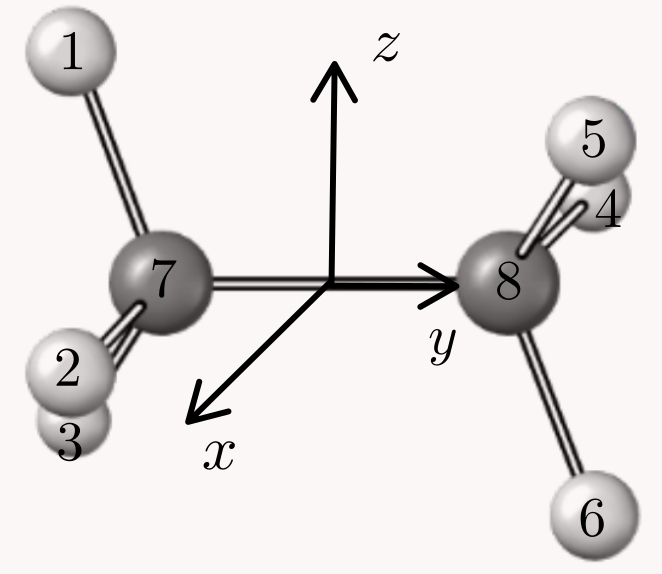
\includegraphics[width=0.3\linewidth]{fig/etano_estrelado.png}
\caption{Etano estrelado C$_2$H$_6$ com seus átomos enumerados.}
\label{fig:etano_estrelado}
\end{figure}

\begin{figure}[H]
\centering
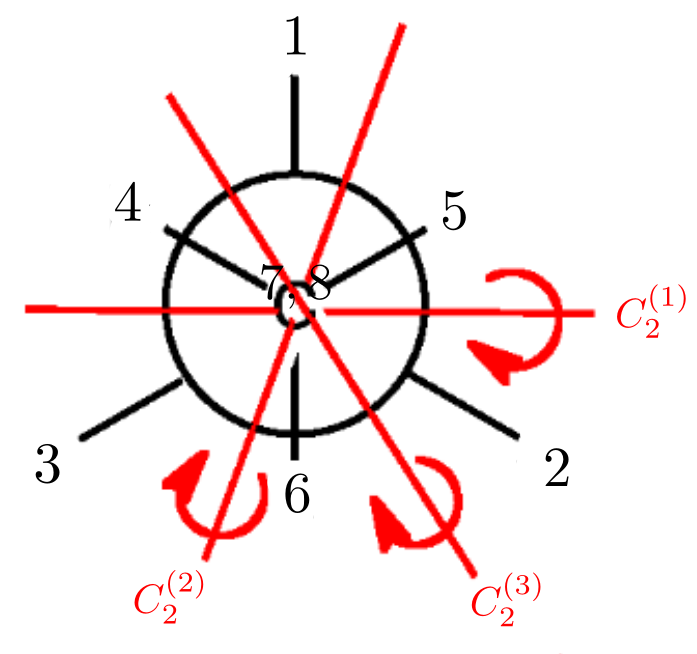
\includegraphics[width=0.3\linewidth]{fig/C2_estrelado.png}
\caption{Eixos de rotação $C_2$ do etano estrelado numa visão onde o eixo $y$ está saindo do plano do papel.}
\label{fig:C2_estrelado}
\end{figure}


Para o etano estrelado, o grupo pontual é o $D_{3d}$. Analogamente ao caso anterior, escrevemos o produto direto
\begin{equation} \label{eq:D3d-direct}
D_{3d} = D_3 \otimes C_{i} =
\{E, C_3, C_3^2, C_2^{(1)}, C_2^{(2)}, C_2^{(3)}\} \otimes \{E, i\} =
\end{equation}
$$
=
\{E, C_3, \underbrace{C_3^2}_{C_3^{-1}}, C_2^{(1)}, C_2^{(2)}, C_2^{(3)},
\underbrace{\sigma_d^{(1)}}_{C_2^{(1)} i},
\underbrace{\sigma_d^{(2)}}_{C_2^{(2)} i},
\underbrace{\sigma_d^{(3)}}_{C_2^{(3)} i},
i,
\underbrace{S_6}_{C_3 i},
\underbrace{S_6^5}_{C_3^2 i}\}.
$$

Seguindo as Figuras \ref{fig:etano_estrelado} e \ref{fig:C2_estrelado}, os elementos ``base'' $C_3, C_2^{(1)}, C_2^{(2)}, C_2^{(3)}, i$ são definidos pelas permutações
$$
C_3
\begin{cases}
\; 1 \to 2 \to 3 \to 1 \\
\; 4 \to 5 \to 6 \to 4
\end{cases}
\Rightarrow \;
C_3 =
\begin{pmatrix}
1 & 2 & 3 & 4 & 5 & 6 & 7 & 8 \\
2 & 3 & 1 & 5 & 6 & 4 & 7 & 8 \\
\end{pmatrix}, \quad
$$
$$
C_2^{(1)}
\begin{cases}
\; 1 \lr 6, \; 2 \lr 5 \\
\; 3 \lr 4, \; 7 \lr 8
\end{cases}
\Rightarrow \;
C_2^{(1)} =
\begin{pmatrix}
1 & 2 & 3 & 4 & 5 & 6 & 7 & 8 \\
6 & 5 & 4 & 3 & 2 & 1 & 8 & 7 \\
\end{pmatrix},
$$
$$
C_2^{(2)}
\begin{cases}
\; 1 \lr 5, \; 2 \lr 4 \\
\; 3 \lr 6, \; 7 \lr 8
\end{cases}
\Rightarrow \;
C_2^{(2)} =
\begin{pmatrix}
1 & 2 & 3 & 4 & 5 & 6 & 7 & 8 \\
5 & 4 & 6 & 2 & 1 & 3 & 8 & 7 \\
\end{pmatrix},
$$
$$
C_2^{(3)}
\begin{cases}
\; 1 \lr 4, \; 2 \lr 6 \\
\; 3 \lr 5, \; 7 \lr 8
\end{cases}
\Rightarrow \;
C_2^{(3)} =
\begin{pmatrix}
1 & 2 & 3 & 4 & 5 & 6 & 7 & 8 \\
4 & 6 & 5 & 1 & 3 & 2 & 8 & 7 \\
\end{pmatrix}.
$$
$$
i
\begin{cases}
\; 1 \lr 6, \; 2 \lr 4 \\
\; 3 \lr 5, \; 7 \lr 8
\end{cases}
\Rightarrow \;
i =
\begin{pmatrix}
1 & 2 & 3 & 4 & 5 & 6 & 7 & 8 \\
6 & 4 & 5 & 2 & 3 & 1 & 8 & 7 \\
\end{pmatrix}, \quad
$$



O grupo $D_{3d}$ é portanto gerado pela função \python{def generate_D3d}.
\begin{Python}
def generate_D3d():
    E = Element(ident(8), r'$E$')
    C3 = Element(Perm([2,3,1,5,6,4,7,8]), r'$C_3$')
    C32 = Element(C3.perm.inv(), r'$C_3^2$')                    # $C_3^{-1}$
    C21 = Element(Perm([6,5,4,3,2,1,8,7]), r'$C_2^{(1)}$')
    C22 = Element(Perm([5,4,6,2,1,3,8,7]), r'$C_2^{(2)}$')
    C23 = Element(Perm([4,6,5,1,3,2,8,7]), r'$C_2^{(3)}$')
    I = Element(Perm([6,4,5,2,3,1,8,7]), r'$i$')
    S6 = Element(C3.perm * I.perm, r'$S_6$')                    # $C_3 i$
    S65 = Element(C32.perm * I.perm, r'$S_6^5$')                # $C_3^2 i$
    Sigma_d1 = Element(C21.perm * I.perm, r'$\sigma_d^{(1)}$')  # $C_2^{(1)} i$
    Sigma_d2 = Element(C22.perm * I.perm, r'$\sigma_d^{(2)}$')  # $C_2^{(2)} i$
    Sigma_d3 = Element(C23.perm * I.perm, r'$\sigma_d^{(3)}$')  # $C_2^{(3)} i$
    D3d = Group([E, C3, C32, C21, C22, C23,
                 Sigma_d1, Sigma_d2, Sigma_d3, I, S6, S65], r'$D_{3d}$')
    return D3d
\end{Python}

Utilizando as mesmas funções e métodos do \python{python} já codadas anteriormente, nosso código retorna a Tabela \ref{tab:mult_D3d} e as classes da equação \ref{eq:D3d-classes}.

\begin{table}[ht]
\caption{Tabela de multiplicação para o grupo $D_{3d}$ da molécula do etano estrelado.}
\centering


\begin{tabular} { |c|c c c c c c c c c c c c | }
\hline
$D_{3d}$ & $E$ & $C_3$ & $C_3^2$ & $C_2^{(1)}$ & $C_2^{(2)}$ & $C_2^{(3)}$ & $\sigma_d^{(1)}$ & $\sigma_d^{(2)}$ & $\sigma_d^{(3)}$ & $i$ & $S_6$ & $S_6^5$ \\
\hline
$E$ & $E$ & $C_3$ & $C_3^2$ & $C_2^{(1)}$ & $C_2^{(2)}$ & $C_2^{(3)}$ & $\sigma_d^{(1)}$ & $\sigma_d^{(2)}$ & $\sigma_d^{(3)}$ & $i$ & $S_6$ & $S_6^5$ \\
$C_3$ & $C_3$ & $C_3^2$ & $E$ & $C_2^{(3)}$ & $C_2^{(1)}$ & $C_2^{(2)}$ & $\sigma_d^{(3)}$ & $\sigma_d^{(1)}$ & $\sigma_d^{(2)}$ & $S_6$ & $S_6^5$ & $i$ \\
$C_3^2$ & $C_3^2$ & $E$ & $C_3$ & $C_2^{(2)}$ & $C_2^{(3)}$ & $C_2^{(1)}$ & $\sigma_d^{(2)}$ & $\sigma_d^{(3)}$ & $\sigma_d^{(1)}$ & $S_6^5$ & $i$ & $S_6$ \\
$C_2^{(1)}$ & $C_2^{(1)}$ & $C_2^{(2)}$ & $C_2^{(3)}$ & $E$ & $C_3$ & $C_3^2$ & $i$ & $S_6$ & $S_6^5$ & $\sigma_d^{(1)}$ & $\sigma_d^{(2)}$ & $\sigma_d^{(3)}$ \\
$C_2^{(2)}$ & $C_2^{(2)}$ & $C_2^{(3)}$ & $C_2^{(1)}$ & $C_3^2$ & $E$ & $C_3$ & $S_6^5$ & $i$ & $S_6$ & $\sigma_d^{(2)}$ & $\sigma_d^{(3)}$ & $\sigma_d^{(1)}$ \\
$C_2^{(3)}$ & $C_2^{(3)}$ & $C_2^{(1)}$ & $C_2^{(2)}$ & $C_3$ & $C_3^2$ & $E$ & $S_6$ & $S_6^5$ & $i$ & $\sigma_d^{(3)}$ & $\sigma_d^{(1)}$ & $\sigma_d^{(2)}$ \\
$\sigma_d^{(1)}$ & $\sigma_d^{(1)}$ & $\sigma_d^{(2)}$ & $\sigma_d^{(3)}$ & $i$ & $S_6$ & $S_6^5$ & $E$ & $C_3$ & $C_3^2$ & $C_2^{(1)}$ & $C_2^{(2)}$ & $C_2^{(3)}$ \\
$\sigma_d^{(2)}$ & $\sigma_d^{(2)}$ & $\sigma_d^{(3)}$ & $\sigma_d^{(1)}$ & $S_6^5$ & $i$ & $S_6$ & $C_3^2$ & $E$ & $C_3$ & $C_2^{(2)}$ & $C_2^{(3)}$ & $C_2^{(1)}$ \\
$\sigma_d^{(3)}$ & $\sigma_d^{(3)}$ & $\sigma_d^{(1)}$ & $\sigma_d^{(2)}$ & $S_6$ & $S_6^5$ & $i$ & $C_3$ & $C_3^2$ & $E$ & $C_2^{(3)}$ & $C_2^{(1)}$ & $C_2^{(2)}$ \\
$i$ & $i$ & $S_6$ & $S_6^5$ & $\sigma_d^{(1)}$ & $\sigma_d^{(2)}$ & $\sigma_d^{(3)}$ & $C_2^{(1)}$ & $C_2^{(2)}$ & $C_2^{(3)}$ & $E$ & $C_3$ & $C_3^2$ \\
$S_6$ & $S_6$ & $S_6^5$ & $i$ & $\sigma_d^{(3)}$ & $\sigma_d^{(1)}$ & $\sigma_d^{(2)}$ & $C_2^{(3)}$ & $C_2^{(1)}$ & $C_2^{(2)}$ & $C_3$ & $C_3^2$ & $E$ \\
$S_6^5$ & $S_6^5$ & $i$ & $S_6$ & $\sigma_d^{(2)}$ & $\sigma_d^{(3)}$ & $\sigma_d^{(1)}$ & $C_2^{(2)}$ & $C_2^{(3)}$ & $C_2^{(1)}$ & $C_3^2$ & $E$ & $C_3$ \\
\hline
\end{tabular}

\label{tab:mult_D3d}
\end{table}


Classes de conjugação do grupo $D_{3d}$ do etano estrelado:
\begin{equation} \label{eq:D3d-classes}
\boxed{
\{ E \}, \;
\{ C_2^{(1)}, C_2^{(2)}, C_2^{(3)} \}, \;
\{ C_3, C_3^2 \}, \;
\{ S_6, S_6^5 \}, \;
\{ \sigma_d^{(3)}, \sigma_d^{(2)}, \sigma_d^{(1)} \}, \;
\{ i \}.
}
\end{equation}

Devido às classes na equação \ref{eq:D3d-classes} do grupo $D_{3d}$ não serem de elementos únicos, o grupo $D_{3d}$ não é abeliano e, por consequência, também não é cíclico.

\pagebreak

\section*{Hexafluoreto de enxofre SF$_6$}

Encontrar os 48 elementos de simetria do grupo $O_h$.

<++>

\pagebreak

\section*{Apêndice: código source do programa em \python{python}} \label{sec:apendice}

\begin{Python}
class Group:    # structure definida como uma lista de 'Element' e o nome do grupo
    def __init__(self, elements, name):
        self.elements = elements
        self.name = name
    def find(self, perm):  # procura o elemento correspondente a uma permutação dada
        for g in self.elements:
            if perm == g.perm:
                return g
        return None
    def printtable(self):  # método que printa a tabela de multiplicação em LaTeX
        elem = self.elements; group_name = self.name; order = len(elem)
        def tabular_string(n):
            s = "|c|"
            while n > 0:
                s = s+"c " if n > 1 else s+"c |"
                n -= 1
            return s
        print(r'\begin{tabular} { %s }' % tabular_string(order)) # tabular do LaTeX
        print(r'\hline')    # linha horizontal
        print(group_name+' ', end='')
        for j in range(order): # printa a primeira linha com os elementos
            if j < order-1:
                print(f'& {elem[j].eqname} ', end='')
            else:
                print(f'& {elem[j].eqname} \\\\')
        print(r'\hline')
        for i in range(order):
            print(f'{elem[i].eqname} & ', end='')  # printa a primeira coluna
            for j in range(order):
                res = self.find(elem[i].perm * elem[j].perm)  # multiplica elementos
                if j < order-1:
                    print(f'{res.eqname} & ', end='')
                else:
                    print(f'{res.eqname} \\\\')
        print(r'\hline')
        print(r'\end{tabular}')

class Element:  # permutacao e o nome
    def __init__(self, perm, eqname):
        self.perm = perm
        self.name = eqname[1:-1]  # remove '\$\$' from latex equation
        self.eqname = eqname

class Perm:
    def __init__(self, L):  # inicialização a partir de uma lista
        self.n = len(L)     # tamanho da lista
        self.list = [i-1 for i in L]  # subtrair 1 para indexar a partir do zero
    def __eq__(self, other):
        return self.list == other.list  # são iguais se as listas são iguais
    def __mul__(self, other):  # multiplicação de duas permutações
        return Perm([self.list[i]+1 for i in other.list])  # composição
    def find(self, j):  # método auxiliar para achar a posição de um número na lista
        for i in range(self.n):
            if self.list[i] == j:
                return i
    def inv(self):  # calcula a inversa de uma permutação
        return Perm([self.find(j)+1 for j in range(self.n)])
\end{Python}

\section*{Apêndice: código source do programa em \python{python}}

\begin{Python}
def ident(n):   # elemento identidade
    return Perm([i for i in range(1, n+1)])

def generate_D3h():
    E = Element(Perm([1,2,3,4,5,6,7,8]), r'$E$')
    C3 = Element(Perm([3,4,5,6,1,2,7,8]), r'$C_3$')
    C32 = Element(C3.perm.inv(), r'$C_3^2$')                            # $C_3^{-1}$
    Sigma_h = Element(Perm([2,1,4,3,6,5,8,7]), r'$\sigma_h$')
    C21 = Element(Perm([2,1,6,5,4,3,8,7]), r'$C_2^{(1)}$')
    C22 = Element(Perm([6,5,4,3,2,1,8,7]), r'$C_2^{(2)}$')
    C23 = Element(Perm([4,3,2,1,6,5,8,7]), r'$C_2^{(3)}$')
    S3 = Element(C3.perm * Sigma_h.perm, r'$S_3$')                      # $C_3 \sigma_h$
    S32 = Element(C32.perm * Sigma_h.perm, r'$S_3^2$')                  # $C_3^2 \sigma_h$
    Sigma_v1 = Element(C21.perm * Sigma_h.perm, r'$\sigma_v^{(1)}$')    # $C_2^{(1)} \sigma_h$
    Sigma_v2 = Element(C22.perm * Sigma_h.perm, r'$\sigma_v^{(2)}$')    # $C_2^{(2)} \sigma_h$
    Sigma_v3 = Element(C23.perm * Sigma_h.perm, r'$\sigma_v^{(3)}$')    # $C_2^{(3)} \sigma_h$
    D3h = Group([E, C3, C32, C21, C22, C23, Sigma_v1,
                 Sigma_v2, Sigma_v3, Sigma_h, S3, S32], r'$D_{3h}$')
    return D3h

def generate_D3d():
    E = Element(ident(8), r'$E$')
    C3 = Element(Perm([2,3,1,5,6,4,7,8]), r'$C_3$')
    C32 = Element(C3.perm.inv(), r'$C_3^2$')                    # $C_3^{-1}$
    C21 = Element(Perm([6,5,4,3,2,1,8,7]), r'$C_2^{(1)}$')
    C22 = Element(Perm([5,4,6,2,1,3,8,7]), r'$C_2^{(2)}$')
    C23 = Element(Perm([4,6,5,1,3,2,8,7]), r'$C_2^{(3)}$')
    I = Element(Perm([6,4,5,2,3,1,8,7]), r'$i$')
    S6 = Element(C3.perm * I.perm, r'$S_6$')                    # $C_3 i$
    S65 = Element(C32.perm * I.perm, r'$S_6^5$')                # $C_3^2 i$
    Sigma_d1 = Element(C21.perm * I.perm, r'$\sigma_d^{(1)}$')  # $C_2^{(1)} i$
    Sigma_d2 = Element(C22.perm * I.perm, r'$\sigma_d^{(2)}$')  # $C_2^{(2)} i$
    Sigma_d3 = Element(C23.perm * I.perm, r'$\sigma_d^{(3)}$')  # $C_2^{(3)} i$
    D3d = Group([E, C3, C32, C21, C22, C23,
                 Sigma_d1, Sigma_d2, Sigma_d3, I, S6, S65], r'$D_{3d}$')
    return D3d

def conjugacy_classes(group):
    classes = set()     # conjunto de classes
    for g in group.elements:
        g_class = set() # classe: conjunto de elementos
        for A in group.elements:
            g_class.add(group.find(A.perm.inv() * g.perm * A.perm)) # $A G A^{-1}$
        g_class = frozenset(g_class)  # frozenset para criar conjunto de conjuntos
        classes.add(g_class)
    return classes

def print_conjclass(cl):
    string = r"\{ "
    for g in cl:
        string += "%s, " % g.name
    string = string[:-2] + r" \}"
    print(string)
\end{Python}

\section*{Apêndice: código source do programa em \python{python}}

\begin{Python}
def main():
    group = generate_D3h()
    #group = generate\_D3d()
    group.printtable()
    classes = conjugacy_classes(group)
    for cl in classes:
        print_conjclass(cl)

if __name__ == '__main__':
    main()
\end{Python}

\end{document}
